%\clearpage
%//==============================--@--==============================//%
%\vspace{-1em}
\subsection{P4 | Velocidade horizontal constante e choque com uma parede}
\label{subsec:P4}

\noindent De modo a manter a discussão sucinta, apresenta-se um modelo simplificado para a interação da bola saltitante---com velocidade horizontal constante---com superfícies verticais. Não será apresentada uma formulação teórica (tal como na \hyperref[sec:intro]{secção intro- dutória}) para este sistema, pelo que são expostas condições mais relaxadas.

\vspace{-1em}
\begin{figure}[H]
    \centering
    \hspace*{-3.75em}\resizebox{0.8\textwidth}{!}{
        \begin{tikzpicture}[node distance = 2.7cm, on grid, auto, transform shape]
            
            \node[state,
                initial below,
                initial text = {\underline{\texttt{Condições iniciais}}},
                fill=orange!20,
                align=center,
                inner sep=0pt] (q_0) 
            {\textit{\underline{Flow}}\\ $\begin{cases} \dot{z} = v_z\\ \dot{v_z} = -g \\ \dot{y} = v_y\\ \dot{v_y} \equiv 0\end{cases}$};
            
            \path [-stealth, thick]
                (q_0) edge[loop right] 
                node[above, yshift = 0.55cm]
                    {$\begin{aligned}&\mkern-24mu\textit{\underline{Superfície horizontal}} \\ &z \le 0 \land v_z < 0 \end{aligned}$}
                node[right, yshift = -0.25cm] 
                    {$\begin{aligned}
                        &\;\, \textit{\underline{Jump}}\\[-0.7ex]
                        v_z &:= -\alpha_z \cdot v_z
                    \end{aligned}$} 
                (q_0)
    
                (q_0) edge[loop left] 
                node[above, yshift = 0.55cm, xshift = -1.25cm]
                    {$\begin{aligned}&\mkern18mu\textit{\underline{Superfície vertical (paredes)}} \\ (y &\le 0 \land v_y < 0)\lor (y \ge P \land v_y > 0) \end{aligned}$}
                node[left, yshift = -0.25cm] 
                    {$\begin{aligned}
                        &\;\, \textit{\underline{Jump}}\\[-0.7ex]
                        v_y &:= -\alpha_y \cdot v_y
                    \end{aligned}$} 
                (q_0);
                
        \end{tikzpicture}
    }
    \caption{Modelo utilizado computacionalmente do novo sistema híbrido.}
    \label{fig:P4-modelo-computacional-sistema-hibrido}
\end{figure}

\vspace{-1em}
\noindent O modelo simplificado pressupõe \underline{independência entre as componentes ortogonais} da velocidade, i.e., colisões com a superfície horizontal atualizam apenas $v_z$ mediante o valor do coeficiente de restituição da superfície, $\alpha_z$; analogamente, as colisões com a superfície vertical atualizam somente $v_y$ consoante um $\alpha_y$.

%\iffalse
\begin{figure}[H]
    \begin{subfigure}[b]{0.5\linewidth}
        \centering
        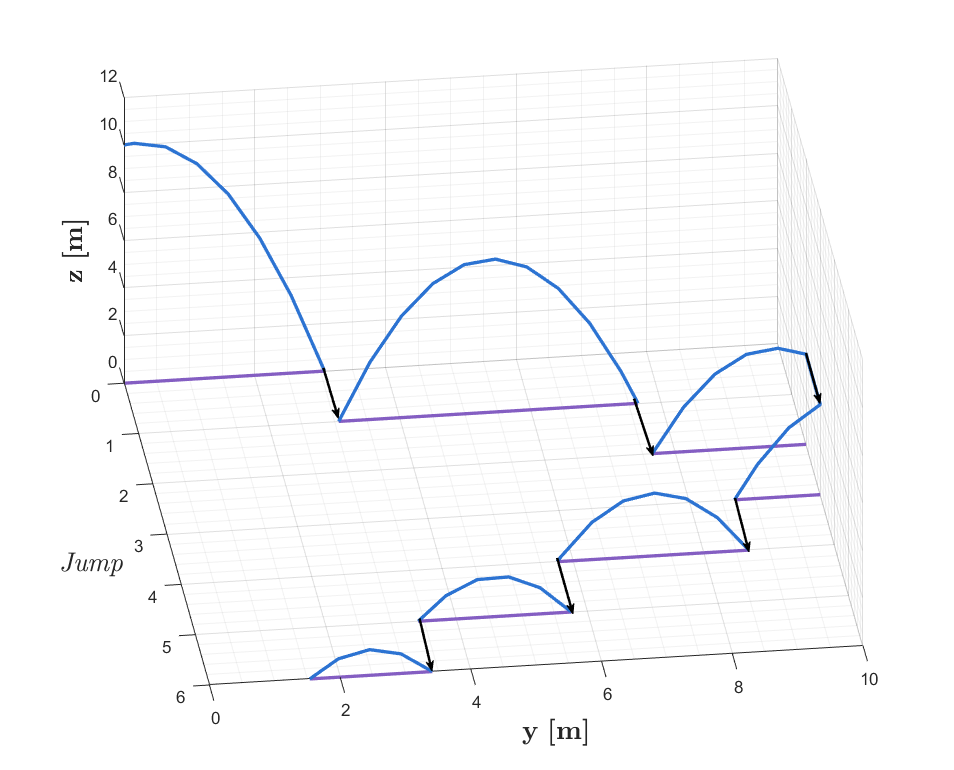
\includegraphics[width=1\linewidth]{img/P4/P4-3dPlot.png}
        \caption{\underline{Trajetória para}:\\ Paredes em $0$ e $P = 10$ m, $z_0 = 10$ m, $v_{z_0} = 0$ ms$^{-1}$, $\alpha_z = 0.8$, $v_y = 2$ ms$^{-1}$ e $\alpha_y = 0.8$.} 
        \label{fig:P4-3dPlot} 
    \end{subfigure}%%
    \begin{subfigure}[b]{0.5\linewidth}
        \centering
        \animategraphics[width=1\textwidth, loop, autoplay]{14}%frame rate
        {img/P4/gif/BouncingBall-}%path to figures
        {0}%start index
        {70}%end index
        \caption{\underline{Trajetória para}:\\ Paredes em $0$ e $P = 5$ m, $z_0 = 10$ m, $v_{z_0} = 30$ ms$^{-1}$, $\alpha_z = 0.8$, $v_y = 2$ ms$^{-1}$ e $\alpha_y = 1$.}
        \label{fig:BouncingBallGif}
    \end{subfigure}%%
    \caption{Visualização da trajetória da massa pontual para duas situações distintas. A \hyperref[fig:BouncingBallGif]{Fig. 11 (b)} é concedida em formato GIF (animada em PDF readers que suportam JavaScript, e.g., Adobe Reader).}
    \label{fig:P4plots}
\end{figure}
%\fi

\vspace{-1em}
\noindent\textbf{\textit{$\rightarrow$ Observações}}
\vspace{-0.5em}
\begin{itemize}
    \item[$\blacktriangle$] A \hyperref[fig:P4-3dPlot]{Fig. 11 (a)} permite vizualizar espacialmente os embates da bola com as super- fícies e os consequentes \textit{jumps} que se sucedem com estes eventos. O resultado final são segmentos da trajetória obtidos com base no período de \textit{flow} que sucede cada \textit{jump}.
    
    \item[$\blacktriangle$] O uso das duas paredes delimita a trajetória da massa puntiforme, como visível na \hyperref[fig:BouncingBallGif]{Fig. 11 (b)}. Esta delimitação permite visualizar com uma maior frequência o efeito da reflexão do movimento horizontal, mantendo a massa pontual \textit{bounded}. Caso não se verificasse \textit{bounded}, a posição tenderia para menos infinito após a primeira colisão vertical, uma vez que não possui aceleração constante no sentido da superfície vertical em $P$.
\end{itemize}

%//==============================--A--==============================//%
%\clearpage
\noindent De modo a explorar a independendência supramencionada entre as componentes ortogonais do sistemas, é estudada a evolução temporal de cada componente. Para uma melhor visualização, foram selecionados os parâmetros: Paredes em $0$ e $P = 2$ m, $z_0 = 10$ m, $v_{z_0} = 15$ ms$^{-1}$, $\alpha_z = 0.8$, $v_y = 2$ ms$^{-1}$ e $\alpha_y = 0.8$.

%\iffalse
\vspace{-1em}
\begin{figure}[H]
    \begin{subfigure}[b]{0.5\linewidth}
        \centering
        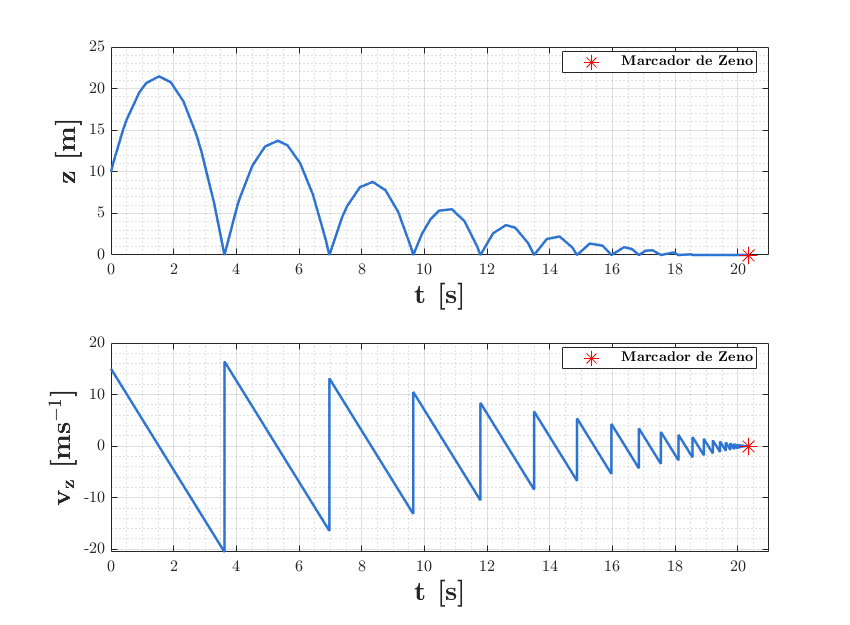
\includegraphics[width=1\linewidth]{img/P4/P4-z}
        \caption{Componente vertical.} 
        \label{fig:P4-z} 
    \end{subfigure}%%
    \begin{subfigure}[b]{0.5\linewidth}
        \centering
        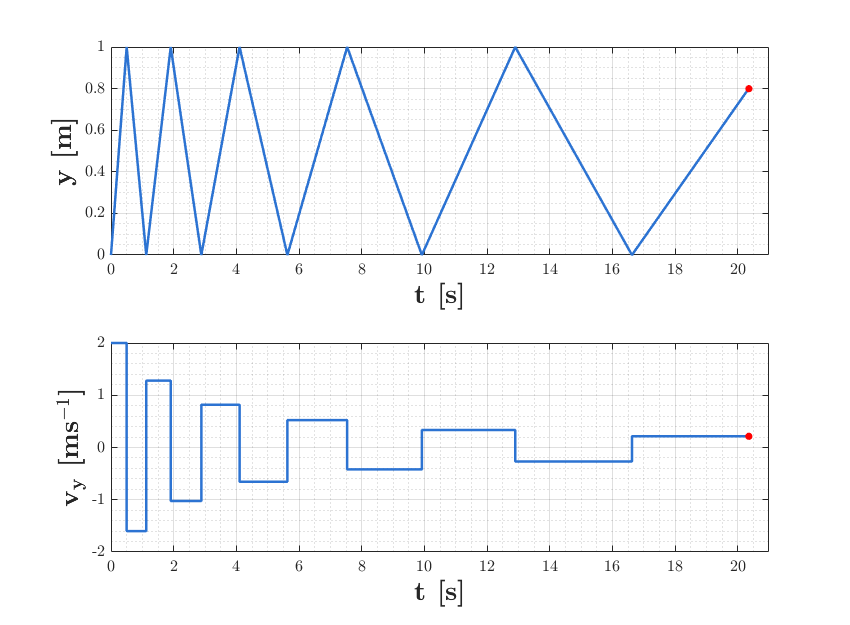
\includegraphics[width=1\linewidth]{img/P4/P4-y}
        \caption{Componente horizontal.} 
        \label{fig:P4-y} 
    \end{subfigure}%%
    \caption{Evolução temporal das componentes verticais e horizontais do sistema. Ao contrário da vertical, os gráficos associados à parte horizontal sofrem uma dilatação ao longo do tempo, dado que as colisões se tornam cada vez menos frequentes, graças à dissipação energética imposta pelo fator $\alpha_y = 0.8$. O marcador (\textcolor{red}{$\bullet$}) denota o fim da simulação.}
    \label{fig:P4-z-y}
\end{figure}
%\fi

%\iffalse
\vspace{-2em}
\begin{figure}[H]
    \begin{subfigure}[b]{0.5\linewidth}
        \centering
        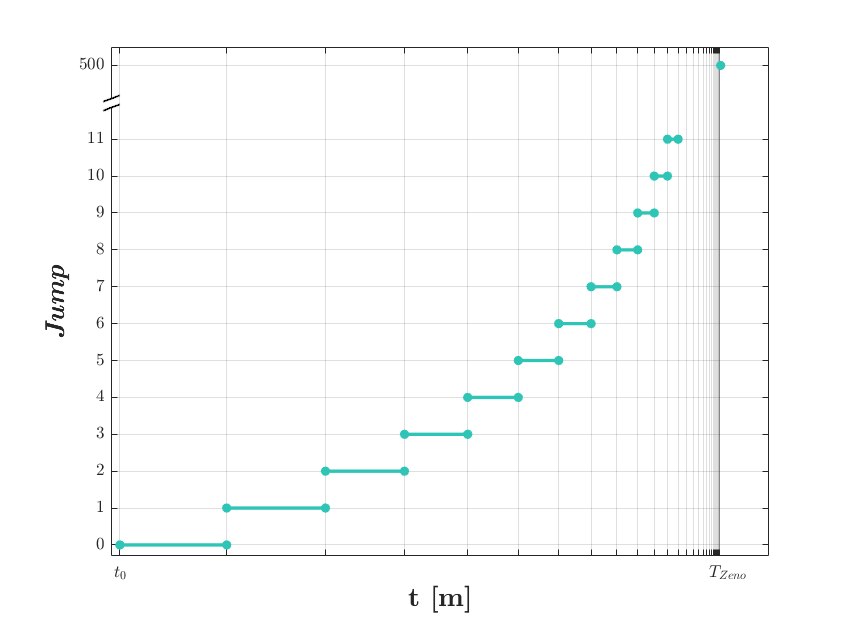
\includegraphics[width=1\linewidth]{img/P4/P4-zeno.png}
        \caption{Componente vertical. Visualização do \hyperref[def:zeno]{efeito de Zeno}. Os intervalos tendem para 0.} 
        \label{fig:P4-zeno} 
    \end{subfigure}%%
    \begin{subfigure}[b]{0.5\linewidth}
        \centering
        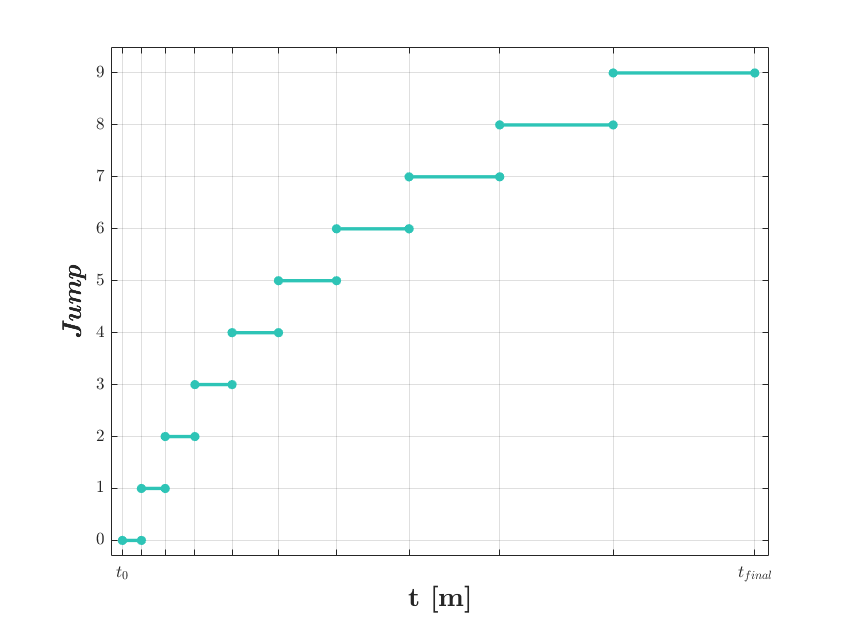
\includegraphics[width=1\linewidth]{img/P4/P4-antizeno.png}
        \caption{Componente horizontal. Efeito da dilatação temporal associada. Os intervalos tendem para infinito.} 
        \label{fig:P4-antizeno} 
    \end{subfigure}%%
    \caption{Evolução da duração dos intervalos de tempo entre colisões com a superfícies horizontal e superfícies verticais. Consoante a discussão da \hyperref[subsec:P1]{secção P1}, verifica-se que $T_{Zeno} =  20.3576$ s, inde- pendente de qualquer influência da componente horizontal, como esperado, dada a ortogonalidade. $t_{final}$ representa o instante final do último período de \textit{flow} completo aparente na \hyperref[fig:P4-y]{Fig. 12 (b)}.}
    \label{fig:P4-zenos}
\end{figure}
%\fi
%//==============================--@--==============================//%